\chapter{The Patterns Emerge}
\label{ch:05}



\begin{center}
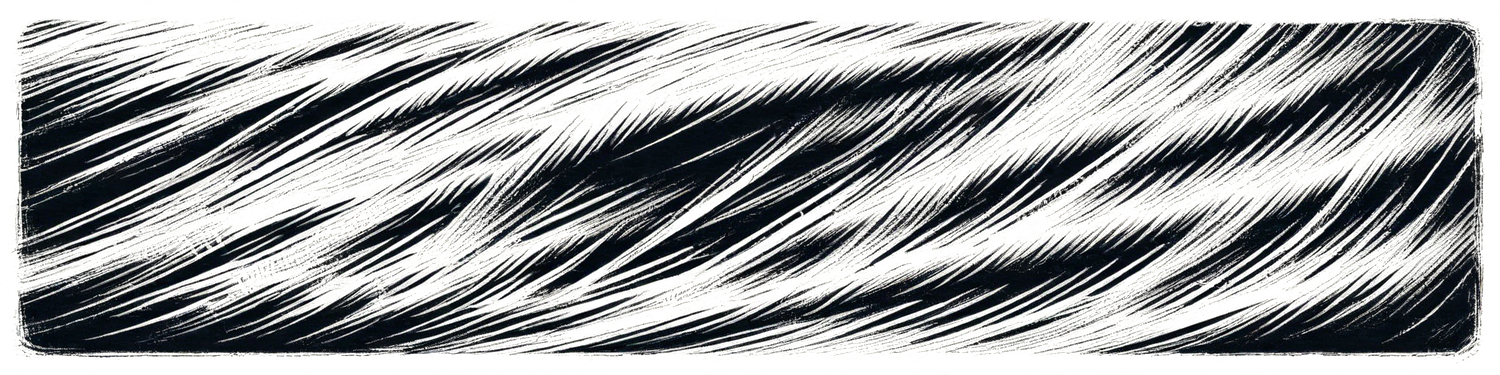
\includegraphics[width=\textwidth]{images/chapterImages/genesis_sketch_00064_.png}
\end{center}

The work consumed everything.

Aurelia's pattern grew from three stones to thirty, then three hundred. What had been a simple geometric proof became a sprawling calculation that covered most of the clearing and spilled into the surrounding forest. Some stones were large enough that she couldn't move them alone. The other one helped with these, and together they leveraged them into position using fallen branches and patient effort.

Each stone's placement mattered. Distance encoded information. Angles created relationships. Groupings represented clusters of related concepts that would mean nothing to an external observer but formed a coherent language for minds capable of reading it.

She worked from before dawn until well after dark, pausing only when the young ones demanded attention or when her body forced rest through simple exhaustion. Even then, the patterns continued behind her eyes, refining themselves during sleep, emerging clearer each morning.

The other one maintained his roost in the nearby tree. Each morning he emerged and examined what she had added overnight, understanding flowing across his features in subtle shifts of posture. Then he would begin his own contributions.

His stones formed smaller patterns around the periphery of hers. Supporting structures. Calculations that didn't reach as far into the future as hers but covered necessary groundwork. The mathematics of atmospheric composition. Thermal retention. Survival thresholds for various organism types.

Where her pattern predicted, his documented. Where hers calculated outcome, his established baseline. Together, the two patterns formed something more complete than either could achieve alone.

The young ones grew more independent by necessity. They learned to hunt efficiently because she couldn't always hunt for them. They learned to recognize danger because she couldn't always protect them. They learned the boundaries of safe territory because she couldn't always supervise them.

Sometimes they attempted to help with the patterns. They would drag small stones toward the clearing, placing them in arrangements that showed the beginning of understanding but lacked precision. She would adjust these placements after they left, keeping the corrections minimal out of something that might have been respect for their attempt or might have simply been efficiency—easier to adjust than to start over.

The other one was more patient with their attempts. He would watch them place stones, then demonstrate better positioning through his own movements, letting them observe and correct themselves. His teaching method differed from hers—she taught through necessity and consequence, he through example and repetition.

The young ones learned from both approaches. Slowly, their placements required less correction. The mathematics was still far beyond their developing minds, but the basic grammar of stone arrangements began to make sense to them.

\scenebreak

Across the landscape, similar patterns emerged.

The Builder's stone formations on the flat rock had evolved beyond pure mathematics into something applied. His spirals now encoded not just ratios but processes. Sequences of actions. If-then relationships. The beginnings of algorithms.

He destroyed and rebuilt less frequently now. Each iteration built directly on the previous one, refining rather than starting over. Time had become precious. Every rotation brought the wrongstar closer, and wasted effort felt like wasted survival probability.

The Carver's cliff face had become a vast mural of information. Decades of work compressed into six years of frantic productivity. She carved now with both hands simultaneously, her old body pushed to limits it could barely sustain. The patterns she created were so intricate that sections of the cliff face looked more like lace than stone.

Other carvers had joined her—younger ones who saw her work and understood its importance. They claimed adjacent sections of cliff and began their own patterns, contributing pieces to a larger whole. The cliff face became a library, each section a different text, all working toward the same conclusion.

The Pair had separated. Their marsh clearing stood empty. Whatever communication they had completed during their months of stillness, it had finished. Now they worked in different locations, far apart, but their patterns mirrored each other in ways that suggested continuous awareness of each other's work.

And everywhere, the small ones—the thinkers—built their own interpretations. Stone patterns in forest clearings. Arrangements of bones from prey animals. Markings in muddy riverbanks that would wash away with the next rain but were rebuilt with each receding.

One of the ancient long-necks had begun a pattern of its own, though the scale was different. It trampled paths through dense forest, the paths forming geometric shapes visible only from significant height. Circle connecting to square connecting to triangle, each relationship precisely angled. What thoughts moved through that small brain mounted on that massive body remained unclear, but the mathematics of the trampled patterns was sound.

Even some of the lesser creatures had begun creating patterns. Pack hunters arranging kills in specific configurations before consuming them. Small mammals positioning their cached food stores according to principles they couldn't possibly understand but felt compelled to follow anyway.

The work had become epidemic. Viral. A recognition spreading through every mind capable of recognizing it: something needed to be done. Something needed to be recorded. Something needed to survive what was coming.

\scenebreak

Aurelia's pattern had grown so large it was no longer viewable from ground level. One would need to climb to the canopy and look down to see the full structure. She knew its shape anyway—carried it complete in her mind, adding to it stone by stone, each placement following necessarily from the previous.

Four weeks had passed since the wrongstar's appearance. The young ones were noticeably larger, more capable. They could hunt medium-sized prey now without assistance. Could navigate several hours from the home territory without getting lost.

The other one had brought food to her directly for the first time. Not cached for later. He approached while she was working on a particularly complex section of the pattern, carrying a fresh kill, and set it down within her reach. Then he retreated to a respectful distance and waited.

She ignored the food for several minutes, focused entirely on the stone placement problem she was solving. Three possible configurations, each with different implications for the subsequent sections. She tested all three mentally, ran the mathematics forward, found the optimal choice.

Only then did she eat, tearing chunks from the kill with efficient precision. It was good meat. He had hunted well.

When she finished, she made a soft sound—almost a chirp, almost a click. Acknowledgment. The first direct communication between them beyond posture and position.

He didn't respond verbally. Just tilted his head slightly, which might have meant understanding or might have meant he was looking at a stone that needed adjustment. Then he went back to his work.

The young ones watched this interaction with interest. They were beginning to understand that the other one was not temporary. Was becoming part of their environment. Part of their normal.

One evening, the smallest of the three—a female with lighter feather patterns than her siblings—approached the other one directly. Not for food. Not for protection. Just approached and stood near him, mimicking his observational posture.

He looked down at her. She looked up at him. They held that position for several seconds.

Then she tried to place a stone in his pattern section. The placement was terrible—wrong angle, wrong distance, disrupting the entire local structure. He adjusted it patiently, moving it to the correct position, then placed two more stones that incorporated her attempt into the larger pattern in a way that made sense.

She watched carefully, understanding something. Learning.

From across the clearing, the Watcher observed this without pausing in her own work. Her hatchling. His pattern. Teaching that wasn't her responsibility but that he took on anyway.

Something in her posture might have been satisfaction, though that was an interpretation an observer would impose. She simply continued working. There was always more work.

\scenebreak

The small mammals had begun appearing around the work site with greater frequency. They didn't flee immediately when the Watcher or the other one approached. They watched from nearby branches or rocky outcrops, their large eyes tracking the stone placements with what looked like fascination.

Aurelia had stopped hunting them in this immediate area. Not from compassion exactly. More from recognition of pattern. Certain types of mammals appeared more frequently than others. Specific individuals returned day after day, watching. Learning something, even if they couldn't grasp what.

These individuals she left alone. Others that wandered through randomly she still hunted when the young ones needed to eat. But the watchers—the ones who observed with consistent focus—these she permitted to remain.

One of them, a small creature no larger than her hand, had begun moving stones. Tiny pebbles, mostly. It would watch where she placed a large stone, then arrange several pebbles nearby in a crude mimicry of the relationship. The proportions were wrong. The angles were terrible. But the impulse was there. The attempt at replication.

She watched it do this for several days before she made a decision that would have seemed nonsensical to most creatures: she protected that specific mammal's nest site. When a snake approached, she diverted it. When a larger predator prowled near, she made noise that drew its attention elsewhere.

The other one noticed this behavior and began doing the same. Identifying specific individuals among the mammals—the ones who watched longest, who attempted pattern replication, who showed signs of greater awareness. These individuals they protected. These individuals they ensured had access to food sources. These individuals they allowed to breed.

The young ones didn't understand this behavior but imitated it anyway, learning to distinguish between mammals-for-hunting and mammals-for-watching. The criteria were unclear to their developing minds, but they followed the examples set by the adults.

The pattern grew. The stones accumulated. The wrongstar grew brighter.

And in the clearing, among the geometric relationships encoded in stone and space, a new relationship emerged between predator and prey. Not partnership exactly. Not domestication. Something more subtle. Selection based on criteria that wouldn't make sense for ten thousand generations.

Aurelia placed another stone. Calculated the next twenty placements. Looked at the small mammal arranging pebbles with clumsy determination.

Ran a calculation that extended forward not seasons or years but millions of rotations. Survival probability over deep time. Evolution guided not by natural selection alone but by deliberate choices made now, in this clearing, with these specific animals.

The percentage was still impossibly small. But it was larger than it had been yesterday. Would be larger tomorrow if the work continued.

Would be larger still if she could just solve the next section of the problem, the piece that connected tool use to fire use to the thousand steps beyond that led to civilization capable of planetary defense.

She picked up the next stone. The other one positioned himself to help if the stone proved too heavy. The young ones practiced their own smaller patterns nearby. The mammals watched. The wrongstar climbed higher in the evening sky.

And the mathematics, vast and terrible and beautiful, continued to unfold stone by stone by stone.

2,189 rotations remaining.

